\documentclass[a4paper,10pt,twoside]{article}
\usepackage[utf8]{inputenc}
\usepackage[french]{babel}
\usepackage[T1]{fontenc}
\usepackage{amsmath}
\usepackage{amsfonts}
\usepackage{amssymb}
\usepackage{graphicx}
\usepackage{multicol}
\usepackage{array}
\usepackage{float}
\usepackage{epstopdf}
\usepackage[justification=centering]{caption}
\usepackage{caption}
\usepackage{subfig}
\usepackage{gensymb}
\usepackage[bottom]{footmisc}
\usepackage{appendix}
\usepackage{pdfpages}
\usepackage{todonotes}
\usepackage{mathpazo}
\usepackage{titleps}
\usepackage{color}
\usepackage{hyperref}
\usepackage[skins]{tcolorbox}
\usepackage{sectsty} 
\usepackage[arrowmos]{circuitikz}
\usepackage{pgfplots}
\usepackage{blindtext}
\usepackage{adjustbox}
\usepackage[inner=2.5cm,outer=2.5cm,top=3cm,bottom=3cm]{geometry}

\graphicspath{{pictures/}}
\setlength\parindent{0pt}
\renewcommand*\rmdefault{ppl}
\newcolumntype{C}[1]{>{\centering\let\newline\\\arraybackslash\hspace{0pt}}m{#1}}
\newcolumntype{R}[1]{>{\raggedright\arraybackslash}p{#1}}
\sectionfont{\large}
\subsectionfont{\normalsize}

% Page style definitions
\newpagestyle{main}{
	\sethead[Club ELEC : Hands-on 1][][]  % even
			{\chaptertitle}{}{Club ELEC : Hands-on 1}
	\headrule
    \setfoot[\thepage][][]
    		{}{}{\thepage}		
}

\newpagestyle{appendix}{
	\sethead[Club ELEC : Annexes][][]  % even
			{}{}{Club ELEC : Annexes}
	\headrule
    \setfoot[\thepage][][]
    		{}{}{\thepage}
    \footrule
}

%----------------------------------------------------------------------------------------
%	TITLE SECTION
%----------------------------------------------------------------------------------------
\title{	
	\vspace{2.5cm}
	\normalfont \normalsize 
	\huge Club ELEC\\ 
	\vspace{2.5cm}
	\huge Projet Audio\\
	\vspace{.25cm}
	\Large HO1 - Contrôle du volume
	\vspace{2.5cm}
	\centering
}

\begin{document}
\renewcommand{\figurename}{Figure}
\renewcommand{\thepage}{\roman{page}}
\setcounter{page}{1}

\pagenumbering{gobble}
\maketitle
\newpage
\pagenumbering{arabic}
\pagestyle{main}

\newpage
\null
\thispagestyle{empty}
\newpage
\clearpage

\setcounter{page}{1}

%%% Introduction (Martin)
\section*{Introduction}
Pendant ce quadrimestre, le Club ELEC vous propose de développer une chaine de conditionnement pour un signal audio, provenant par exemple d'un ordinateur, smartphone, etc. Pour ce faire, le développement du circuit se déroulera en 3 phases, chacune correspondant à une séance de hands-on proposée par le club.

\begin{itemize}
	\item[-] HO1: Contrôle du volume sonore.
	\item[-] HO2: Filtrage du contenu fréquentiel.
	\item[-] HO3: Distortion du signal audio.
\end{itemize}

%%% Objectifs du HO1 (Martin)
\section*{Objectifs}
% Objectifs: prise en main du micro et du signal sonore, notion AC/DC, utilisation de l'oscilloscope, découplage AC

Les objectifs du premier hands-on sont:

\begin{itemize}
	\item[-] De se familiariser avec le matérial de base (breadboard, multimètre, oscilloscope) et les composants de base (résistances, capacités, amplificateurs opérationnels, composants intégrés) propres à l'électronique.
	\item[-] De comprendre le fonctionnement du micro qui assure la transduction du signal sonore en signal électrique.
	\item[-] De faire le lien entre le signal obtenu et son contenu fréquentiel afin de comprendre la notion de filtrage.
	\item[-] De comprendre la notion AC/DC et le découplage AC.
	\item[-] D'implémenter en pratique la première partie du circuit (micro, filtre et découplage).
\end{itemize}

\begin{figure}[!ht]
	\centering
	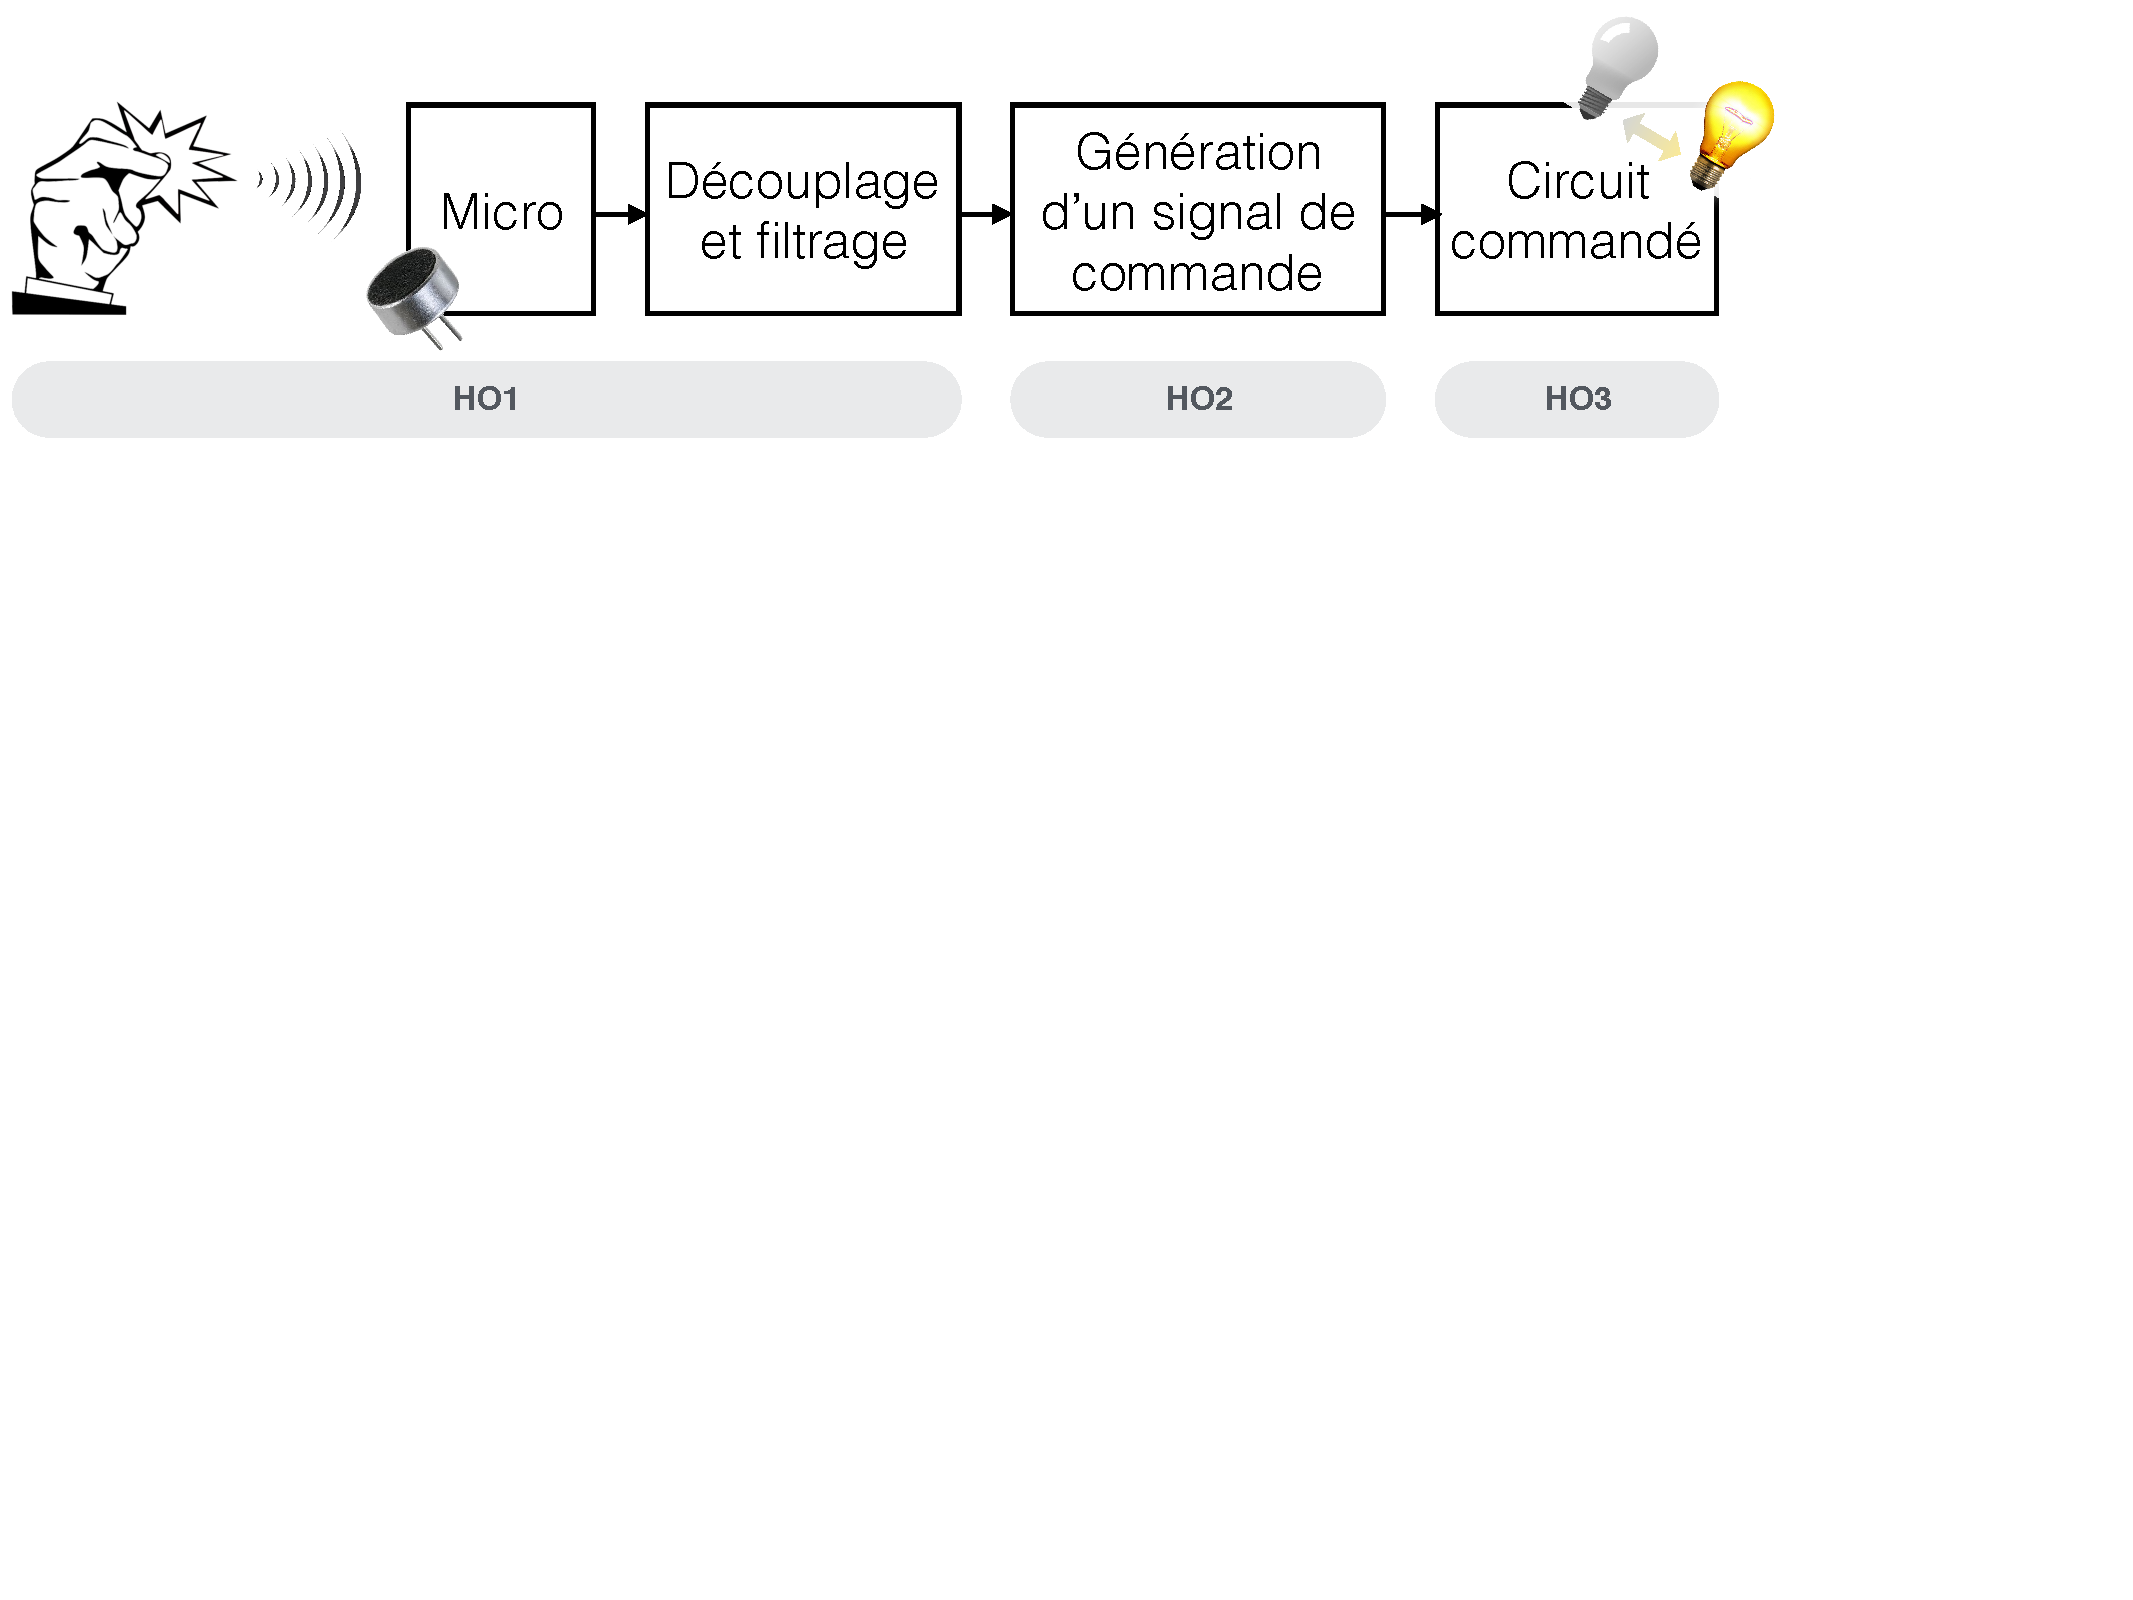
\includegraphics[width=.75\textwidth]{figures/SchemaBloc.pdf}
	\caption{Schéma-bloc du circuit.}
	\label{fig:block-diagram}
\end{figure}

Le schéma-bloc du circuit est présenté à la Figure \ref{fig:block-diagram}. Les ondes acoustiques générées par le claquement de doigt sont captées par le micro qui les transforme en un signal électrique (transduction). Ce signal est ensuite découplé et filtré à l'aide d'un filtre RC, comme présenté plus loin dans ce document. La génération d'un signal de commande propre ainsi que l'implémentation d'un circuit commandé seront abordées plus en détail dans les prochain hands-on.


\newpage 

%%% Explication détaillée des blocs du circuit
\section*{Description du circuit}
\begin{figure}[ht!]
	\centering
	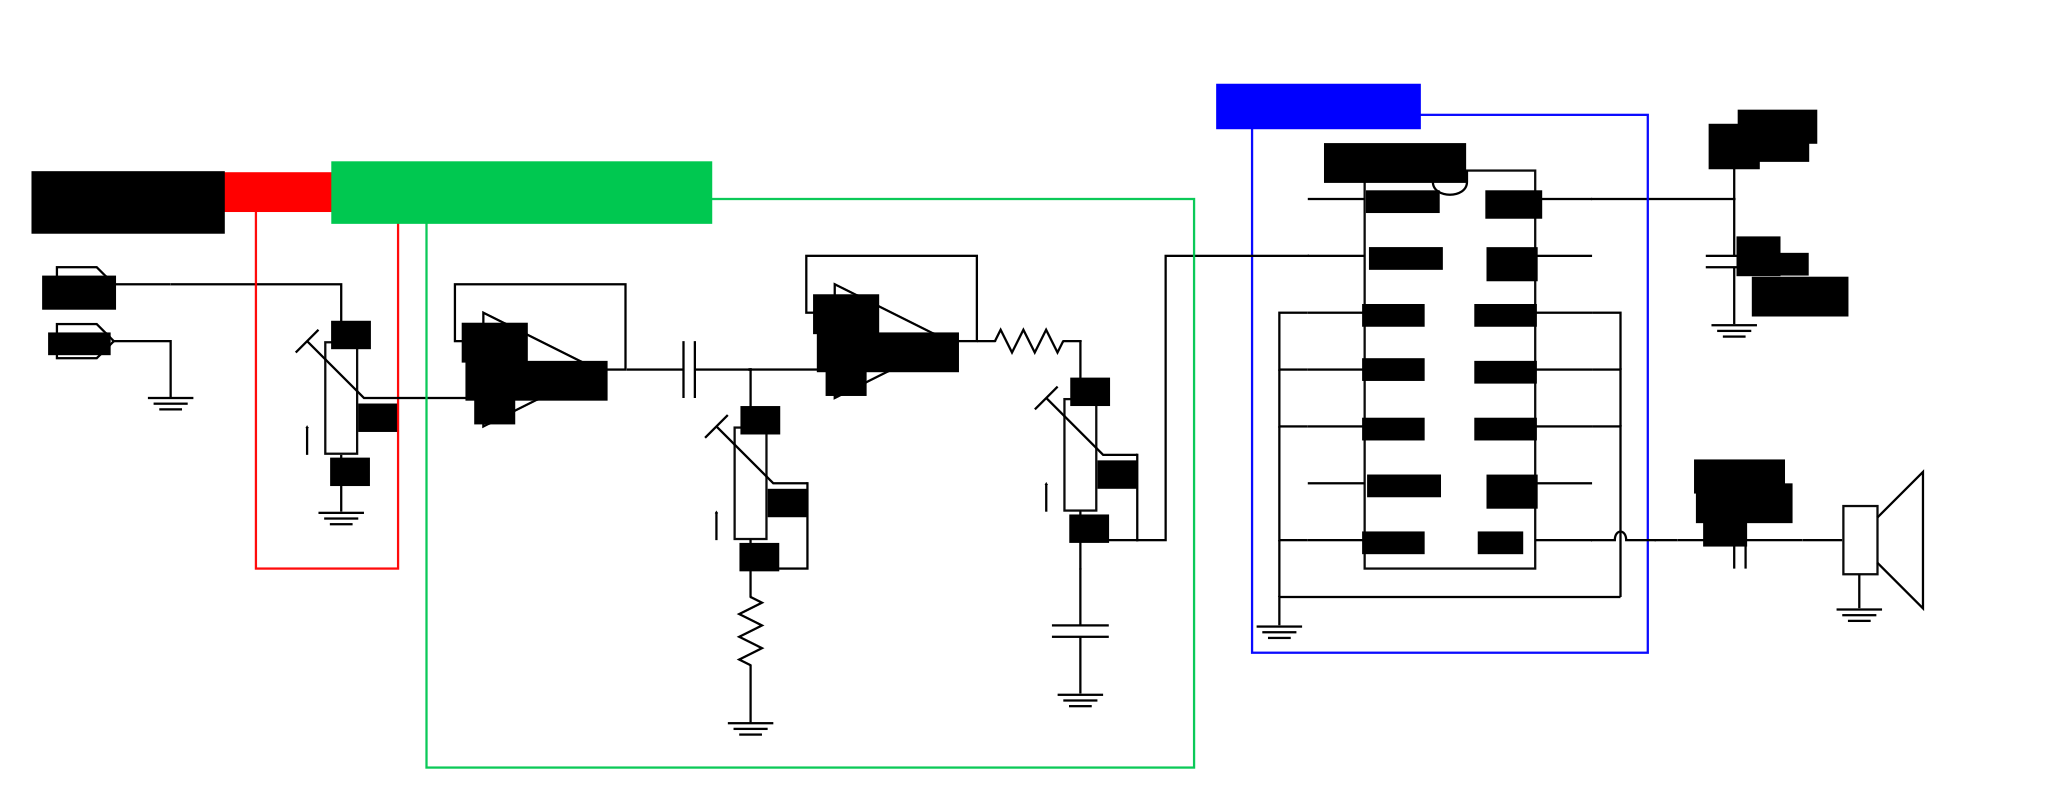
\includegraphics[width=\textwidth]{schematics}
	\caption{Schématique du circuit.}
	\label{fig2:schematics}
\end{figure}

Le schématique du circuit modifié est présenté à la Figure \ref{fig2:schematics}. En partant de la gauche, le signal d'entrée fourni par le câble jack à la borne IN1 passe d'abord dans le bloc de filtrage. Les filtres ont été implémentés sur base de topologies passe-haut et passe-bas passives, c'est-à-dire qu'elles n'utilisent pas d'amplificateur opérationnel. Pour éviter que l'impédance d'entrée (resp. sortie) des blocs suivants (resp. précédents) ait un impact sur le comportement des filtres, ceux-ci sont isolés du reste du circuit par des montages suiveurs, à savoir un amplificateur opérationnel avec une rétroaction unitaire sur la borne négative.Le signal est ensuite transmis au bloc de distorsion (de type overdrive/clipper), inspiré de la pédale appelée \textit{Dan Armstrong's Blue Clipper}. Le détail de ce circuit est présenté à la Figure \ref{fig3:clipper}. Ce bloc inclus également le contrôle du volume, implémenté par un diviseur résistif. Enfin, le signal est amplifié puis transmis au haut-parleur.

% Breadboard (Maxime)
\subsection*{Breadboard}
% Subsection on breadboard

Pour le prototypage de circuits électroniques, on utilise généralement une \emph{breadboard} (ou platine d'expérimentation/prototypage). Il s'agit d'une "plaquette à trous", dans lesquels on peut insérer des fils et des composants pour construire un petit circuit électronique. Un exemple de breadboard se trouve sur la Figure \ref{fig:breadboard_pic}.

Les trous d'une breadboard ne sont pas isolés les uns des autres, ils sont connectés en colonnes ou en lignes, comme illustré sur la Figure \ref{fig:breadboard_conn}. Généralement, les deux premières et les deux dernières colonnes de trous, assignés des signes + et -, sont utilisées pour distribuer les signaux d'alimentation (0V et 5V par exemple). Les lignes de trous au milieu sont plutôt utilisées pour connecter et placer le coeur du circuit.

Comme une breadboard ne nécessite aucune soudure, elle permet de prototyper et débugger rapidement un circuit électronique. Elle est également totalement réutilisable : si un circuit monté sur breadboard n'est plus utilisé, il peut être enlevé facilement en sortant les fils et composants des trous, et la breadboard peut alors être utilisée pour le prototypage d'un autre projet. La breadboard est donc très pratique, mais malheureusement, tous les composants ne peuvent pas y être connectés.\\

\begin{minipage}[t]{.49\textwidth}
	\centering
	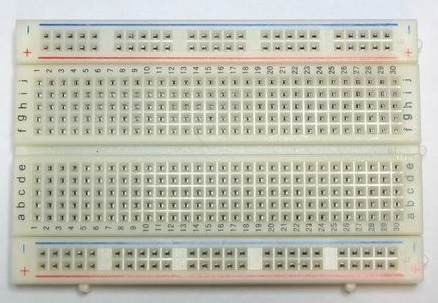
\includegraphics[width=.6\textwidth,angle=90]{figures/breadboard_picture.jpg}
	\captionof{figure}{Photo d'une breadboard.}
	\label{fig:breadboard_pic}
\end{minipage}
\hfill
\begin{minipage}[t]{.49\textwidth}
	\centering
	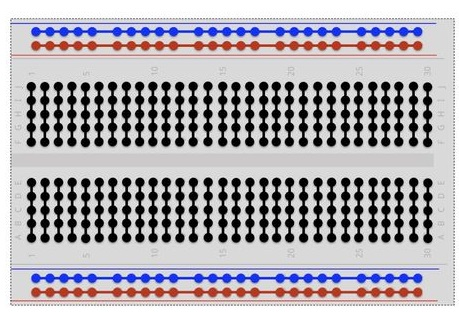
\includegraphics[width=.6\textwidth,angle=90]{figures/breadboard_connections.jpg}
	\captionof{figure}{Connexions des trous d'une breadboard.}
	\label{fig:breadboard_conn}
\end{minipage}
\vspace{1cm}

% Câble jack
\subsection*{Connecteur jack}
% Subsection on jack

Le premier élément nécessaire pour ce hands-on est un \emph{connecteur jack femelle}, tel celui de la Figure \ref{fig:jack_pic}. Ce connecteur permet d'amener les signaux audio sur la breadboard, en y connectant une source audio (smartphone, ordinateur ou autre) via un câble jack mâle-mâle. Malheureusement, les connecteurs jacks ne peuvent pas être insérés tels quels dans les breadboards. Cela peut être réolu simplement via la soudure de quelques fils.\\

\begin{minipage}[c]{\textwidth}
	\centering
	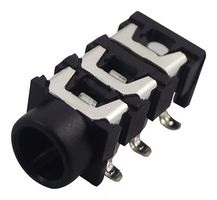
\includegraphics[width=0.3\textwidth]{figures/jack.jpg}
	\captionof{figure}{Photo du connecteur jack femelle.}
	\label{fig:jack_pic}
\end{minipage}
\vspace{1cm}

% Diviseur résistif
\subsection*{Diviseur résistif}
% Subsection on resistive divider

Pour changer le volume, on utilise un diviseur résistif. Une simple résistance variable, appelée aussi \emph{potentiomètre}, fait l'affaire. Une photo de potentiomètre se trouve à la Figure \ref{fig:potentiometre_pic}.\\

Un potentiomètre est un composant à 3 accès (à 3 pattes) qui possède une molette qui se tourne, par exemple avec un tournevis. Le schéma d'un potentiomètre est renseigné à la Figure \ref{fig:potentiometre_sch}. Entre les deux accès les plus éloignés $\alpha$ et $\gamma$, il y a une résistance fixe valant $R_{\alpha\gamma} = R_{\alpha\beta}+R_{\beta\gamma}$, de par exemple $1k\Omega$. L'unité de $1\Omega$ (ohm) correspond à une chute de tension de $1V$ (volt) lorsqu'un courant de $1A$ (ampère) traverse la résistance.\\

En tournant la molette dans un sens ou dans l'autre, l'on change les valeurs des résistances $R_{\alpha\beta}$ et $R_{\beta\gamma}$ (mais leur somme reste fixe). En prenant le noeud $\gamma$ comme référence (à la masse), la tension au noeud $\beta$ est une fraction de la tension du noeud $\alpha$ et peut être ajustée à la valeur désirée grâce à la molette. Dans le contexte du son, cela revient à contrôler son volume.\\

\begin{minipage}[c]{0.45\textwidth}
	\centering
	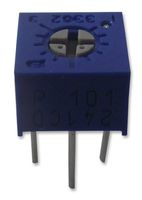
\includegraphics[width=0.4\textwidth]{figures/potentiometre_picture.jpg}
	\captionof{figure}{Schéma d'un potentiomètre.}
	\label{fig:potentiometre_pic}
\end{minipage}
\hfill
\begin{minipage}[c]{0.45\textwidth}
	\centering
	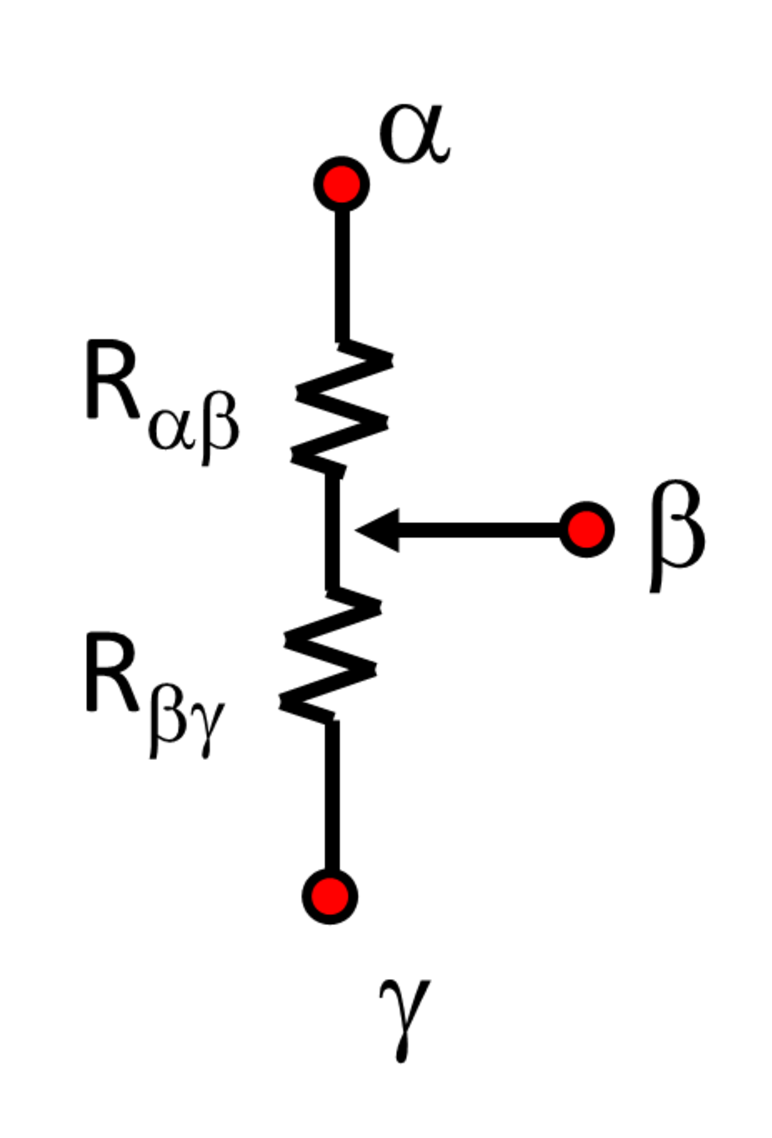
\includegraphics[width=0.4\textwidth]{figures/potentiometre.pdf}
	\captionof{figure}{Schéma d'un potentiomètre.}
	\label{fig:potentiometre_sch}
\end{minipage}
\vspace{1cm}

\newpage

% Amplification
\subsection*{Amplificateur de puissance}
% Subsection on audio amplifier

Un \emph{amplificateur audio} est nécessaire pour pouvoir ressortir le son sur un baffle ou un buzzer. Pour cela, on a à disposition des circuits intégrés à 14 pattes (modèle LM380N de chez Texas Instruments). Le chip LM380N choisi est montré en photo sur la Figure \ref{fig:ampli_pic}.\\

Le sens du boîtier de l'amplificateur est renseigné avec une petite encoche, généralement placée vers le haut. Chaque patte/pin du circuit a un but précis et un nom, renseigné sur la Figure \ref{fig:ampli_pins}. Par exemple, le circuit est alimenté avec du +15V, à connecter sur sa pin 14 ($V_s$). La masse ou 0V, aussi nommée $GND$, doit être connectée à plusieurs pins (3, 4, 5, 7, 10, 11, 12), notamment pour une question de dissipation de puissance. Il ne faut pas oublier qu'il s'agit d'un amplificateur audio qui nécessite quand même un peu de puissance. Les autres connexions sont à retrouver sur le schéma général du circuit à la Figure \ref{fig:schematics}.\\

\begin{minipage}[c]{.49\textwidth}
	\centering
	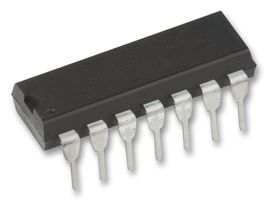
\includegraphics[width=0.6\textwidth]{figures/LM380N_picture.jpg}
	\captionof{figure}{Photo de l'amplificateur audio LM380N.}
	\label{fig:ampli_pic}
\end{minipage}
\hfill
\begin{minipage}[c]{.49\textwidth}
	\centering
	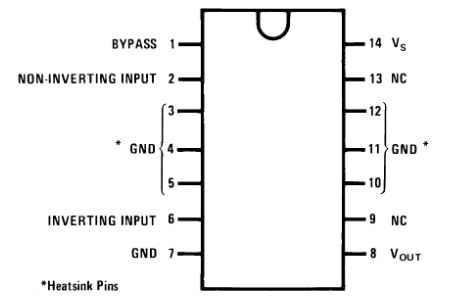
\includegraphics[width=\textwidth]{figures/LM380N_sch.jpg}
	\captionof{figure}{Nom des pattes de l'amplificateur audio LM380N.}
	\label{fig:ampli_pins}
\end{minipage}
\vspace{1cm}

% Baffle/Piézo
\subsection*{Baffle}
% Subsection on buzzer/woofer

Enfin, le dernier composant nécessaire est un \emph{baffle} ou un \emph{buzzer}. Ces éléments sont représentés sur les Figures \ref{fig:woofer_pic} et \ref{fig:buzzer_pic} respectivement. Le rôle de ces composants est de transformer un signal électrique (tension/courant) provenant de l'amplificateur audio, en signal audio (ondes sonores, audibles par nos oreilles humaines). Une capacité de découplage est nécessaire également, entre le baffle/buzzer et l'amplificateur audio, pour éviter de trop large pics de courant qui peuvent endommager l'amplificateur.\\

\begin{minipage}[c]{0.45\textwidth}
	\centering
	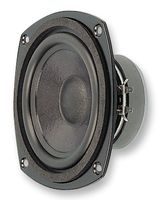
\includegraphics[width=0.4\textwidth]{figures/woofer_picture.jpg}
	\captionof{figure}{Image d'un baffle.}
	\label{fig:woofer_pic}
\end{minipage}
\hfill
\begin{minipage}[c]{0.45\textwidth}
	\centering
	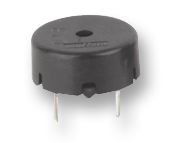
\includegraphics[width=0.4\textwidth]{figures/buzzer_picture.jpg}
	\captionof{figure}{Image d'un buzzer.}
	\label{fig:buzzer_pic}
\end{minipage}
\vspace{1cm}

\end{document}